% !TeX root = ../main.tex

\chapter{绪论}

\section{系统开发背景}
半个世纪以来,集成电路产业伴随着摩尔定律一路高歌猛进,为人类进入信息化时代提供了强大的算力支撑,芯片俨然已经成为信息时代的原油。在如今逆全球化的浪潮中,芯片行业首当其冲,成为了大国博弈的前沿战场。我国的集成电路产业经过了几十年的发展,在某些应用领域也取得了不错的成绩,但在高性能处理器以及芯片设计的关键技术中,仍然面临着巨大的挑战\cite{huzhenbo,huzhenbo1}。不管是2018年中美贸易战中"中兴事件"和"华为事件"的发生,还是其他国家对我国实行的禁运政策,都让我国在市场竞争中处于下风,除了光刻机等硬件生产设备,在工业软件乃至指令集架构等领域,都存在"卡脖子"的现象。


作为软硬件之间至关重要的接口,指令集架构是处理器的灵魂。长期以来,主流的指令级架构作为少数大公司的知识产权,几乎垄断了全球的芯片设计与制造行业,成为绕不开的技术壁垒。不过近年来随着部分开源的指令级架构的诞生,这一局面有望被打破。RISC-V作为一款完全开源的指令集架构,在众多开源指令集架构中脱颖而出,不仅是因为其设计理念先进,采用模块化设计的方案,而且因为它开放,包容,提供了高度灵活的配置空间,在积极拥抱开源软件的今天,RISC-V已经成为未来的主流架构,随着RISC-V开源社区的日益壮大,更多的芯片设计厂商选择RISC-V作为其指令集架构,指导芯片的设计生产\cite{包云岗2022开源芯片生态技术体系构建面临的机遇与挑战}。

% 在集成度越来越高的今天,面对数千万乃至上亿晶体管的规模,那种“设计硬件原型-实现-评估-改进-再实现”的模式已经无法满足现代设计应用的需求\cite{jichengdu}。
% 有研究表明,如果在CPU的方案论证和设计阶段,没有及时发现问题与瓶颈,将会使后续的工作变得更为困难且代价更加高昂。因此,在开发一个新的体系结构处理器时,为了确保处理器功能特性和性能参数达到设计的预期目标,对体系结构进行验证是一个必不可少的步骤\cite{buzhou}。
随着摩尔定律的减缓,在如今的集成度面前,传统的“设计硬件原型-实现-评估-改进-再实现”的芯片开发模式已然落伍\cite{jichengdu}。有研究表明,在实际的芯片开发项目中,如果在前期方案论证阶段没有体系结构模拟器的支持,将很难及时发现设计的缺陷和性能瓶颈,导致后期的工作变得异常困难,且会伴随高昂的代价\cite{buzhou}。除此之外,在芯片开发后期,软硬件适配工作作为测试的重点,往往也需要模拟器环境的支持\cite{黄聪会2012软件移植理论与技术研究,butko2012accuracy},厂商可以根据自身产品特性,设计相应的性能或功能模拟器,并在此基础之上进行软件移植工作和前期软硬件设配工作,以此来提高芯片验证与测试工作的效率。从经济成本和时间成本的角度来看,体系结构模拟器都可以为芯片设计与验证工作提供极大的便利。相较于一些主流指令集架构,当前RISC-V的软件生态尚不完善,各类软件的RISC-V移植工作正在开源社区如火如荼地进行中,对于芯片设计和开发厂商,系统软件的开发移植更是重中之重。因此开发一款符合自身产品特性的RISC-V模拟器将成为贯穿芯片开发周期的一项重要的软件工程。


\section{国内外发展现状}
龙芯中科技术有限公司在龙芯2号处理器研发过程中,开发了模拟器ICT-Godson\cite{gao2007simos},对硬件进行了细粒度的模拟,能够精确地模拟芯片开发过程中的所有硬件信号和行为,但是由于模拟精度过高,导致模拟器执行速度太慢,难以高效地进行辅助工作。因此,基于开源模拟器Simple-Scalar\cite{austin2002simplescalar},龙芯中科公司重新实现了Sim-Godson模拟器\cite{zhang2007sim},该模拟器摒弃了细粒度的硬件仿真,采用执行驱动的组织方式,以及模块化的设计,可以支持时序模拟和功能模拟\cite{zhang2007sim},相较于前一版的模拟器性能得到了极大的提升。使用该模拟器可以直接加载目标程序的二进制可执行文件,通过功能模拟对目标机器进行微结构性能探索\cite{desikan2001sim}。
% 龙芯中科技术有限公司在使用模拟器辅助处理器设计的文献中提到\cite{zhang2007sim,gao2007simos},在龙芯2号处理器研发的早期,开发了模拟器ICT-Godson,由于该模拟器对硬件模拟过于详细,导致其速度和灵活性不足。因此,龙芯基于开源模拟器Simple-Scalar\cite{austin2002simplescalar}重新设计实现了Sim-Godson模拟器\cite{zhang2007sim}。和ICT-Godson模拟器相比,Sim-Godson运行速度更快、灵活性更高,并且支持大程序评估\cite{zhang2007sim}。Sim-Godson可以支持时序模拟和功能模拟,可以直接加载二进制可执行程序进行模拟,该模拟器主要用于处理器核的微结构性能探索。
% 虽然借用了Simple-Scalar的基础模块,但Sim-Godson对其进行了大量修改定制,使其能够高精准地对龙芯2号处理器核微结构进行模拟。基于Simple-Scalar中自带的指令集仿真器和I/O仿真器进行执行加速,其速度可以达到0.5MIPS(million instructions per second)。经过详细校准,Sim-Godson模拟器与ICT-Godson的误差平均不到5\%\cite{zhang2007sim}。类似地,基于Simple-Scalar进行二次开发的模拟器还有Sim-alpha\cite{desikan2001sim}。

Gem5是一款开源的系统级体系结构模拟器,它结合了CPU模拟框架M5和内存时序模拟器GEMS的特点,是一款具有多种执行模式的事件驱动模拟器\cite{许鹏2006一种应用于嵌入式系统中断控制},Gem5能够模拟多种不同架构的处理器,包括Alpha、ARM、X86、SPARC、MIPS等,近年来也支持了RISC-V架构,借助于其开源的强大合作能力,Gem5不断完善自身,在工业界和学术界都极受欢迎。Gem5的灵活性依赖于其面向对象的设计,85\%的Gem5源码由C++编写,在Gem5中可以选择不同的指令集架构和CPU模型。对于部分指令集架构,Gem5支持全系统模式(Full System)运行,在该模式下,Gem5可以运行操作系统,这样也就可以进行中断、异常、特权级别、I/O等的模拟。


IBM在处理器开发的不同时期,使用不同类型的体系结构模拟器进行辅助。在前期设计与规划时期,使用Mambo\cite{boh}模拟器的时钟精确模式进行微结构探索和粗粒度微结构定义,该阶段体系结构模拟器采用踪迹驱动方式\cite{ceze2003full},主要运行和研究用户态应用,对处理器的产品竞争力进行横向比较研究\cite{kistlerexperiences}。在微结构设计实现期间,IBM使用基于公司内部专用“T”语言\cite{asaad2012cycle,chaix2019implementation}编写的时钟精准模拟器M1进行详细模拟\cite{kistlerexperiences},如图~\ref{fig:IBM}所示。M1是以Mambo模拟器或者硬件上抓取的踪迹作为输入,并且可以收集非常详细的微结构数据进行性能评估\cite{magnusson2002simics}。
\begin{figure}[h]
  \centering
  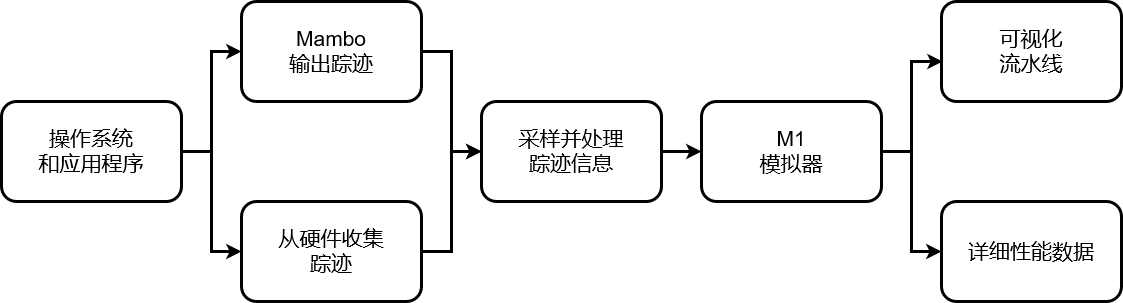
\includegraphics[width=1.0\textwidth]{mambo.png}
  \caption{IBM体系结构模拟器框架}
  \label{fig:IBM}
\end{figure}  


目前RISC-V开源社区的体系结构模拟器有Spike, Gem5, Qemu\cite{bellard2005qemu}等,这一类模拟器能够对部分RISC-V开源架构如BOOM\cite{celio2016berkeley}进行模拟,对于新手熟悉RISC-V有很大的帮助。Spike是一款基于解释型的RISC-V指令集模拟器,能够提供指令级别的仿真,跟开源社区Riscv-Tools里的pk(proxy kernel)和fesrv(front-end server)结合能够完成全系统的模拟,并且能够提供命令行的单步调试。Qemu是一款基于编译型的模拟器\cite{varga2010omnet++},直接对RISC-V二进制流进行翻译,模拟速度接近宿主机。在此类RISC-V模拟器上也能够进行软件移植工作,主要是基于Linux内核的应用软件移植。
% 为了加速M1模拟器的执行速度,需要对所抓取的踪迹进行取样,同时为了方便调试,M1支持微结构性能数据可视化功能。在处理器验证阶段,IBM使用Mambo作为处理器验证参考模型辅助进行验证,此阶段Mambo可以为处理器功能正确性提供参考结果。Mambo模拟了所有处理器的功能特征,把某些性能相关的微结构维护操作(例如cache维护类指令)翻译成空(nop)操作,对于计算类指令产生准确的结果,并精准追踪处理器寄存器的状态变化,同时支持指令撤销操作,为处理器验证提供参考。IBM基于Mambo模拟器曾发现PowerPC CPU的一个控制寄存器存在竞争条件,使得该设计错误在流片之前就被发现并修改。在该阶段,IBM还使用自研的由多个FPGA(field programmable gate array)组成的VHDL(very-high-speed integrated circuithardware description language)仿真加速器Twinstar\cite{asaad2012cycle}进行处理器综合验证。Twinstar是时钟精准的仿真加速器,其推进方式是事件驱动模式,可以对整个处理器芯片进行仿真,以二进制程序作为输入,还支持详细的指令踪迹和处理器状态的实时追踪。该平台运行速度可以达到4MHz并可以运行未经修改的系统软件。类似Twinstar的验证平台还有帕拉丁\cite{chaix2019implementation}等。
% 在系统软件开发方面,IBM基于Mambo(加速模式),Simics\cite{magnusson2002simics},BGLsim\cite{ceze2003full}等多种平台,在流片之前就开始进行固件、操作系统、虚拟机管理器等软件的早期开发。IBM基于Mambo模拟器曾开发了K42操作系统,在芯片可用之后1周内就启动了操作系统\cite{boh}。IBM基于BGLsim-multi\cite{ceze2003full}平台和基于OMNeT++\cite{varga2010omnet++}开发的MARS(message passing interface application replay simulation)模拟平台还可以对机群网络相关的功能进行模拟,模拟器由可执行程序或者踪迹驱动\cite{许鹏2006一种应用于嵌入式系统中断控制},其中MARS平台还可以对MPI(message passing interface)类应用进行调优。



\section{本文主要工作}
为了加快芯片开发项目中的系统软件开发过程,以及辅助进行处理器验证,本文从RISC-V芯片开发项目工作流程入手,设计并实现了一款针对RISC-V体系结构的指令集功能模拟器,可以使得芯片开发团队脱离硬件平台并行地进行系统软件移植,开发和测试工作,本模拟器提供对真实硬件的功能模拟,以及丰富的调试手段,缩短软件开发周期,辅助处理器验证。主要完成的工作如下:


(1)参照RISC-V用户手册,特权级架构文档,以及实际的硬件设计方案,对RISC-V架构处理器进行功能建模,参照硬件设计团队的Chisel代码对RISC-V标准拓展指令集共196条指令进行C++功能函数模拟,结合系统软件开发人员的需求,确定指令集模拟器的模拟策略,规划具体功能模块的边界,采用面向对象的方法进行模块设计。


(2)实现RISC-V指令集模拟器前后端模块,包括预加载模块,CPU和总线模块,中断控制器模块,调试和UI模块。设计并实现平台级中断控制器和部分外设模拟,可以直接在模拟器平台上进行外设驱动的适配;结合实际项目需求,实现UI可视化界面进行交互调试,进一步加强模拟器的易用性。在实际的芯片开发项目中帮助团队进行系统软件开发工作,并对处理器进行辅助验证。


本人负责的主要工作有模拟器前后端整体框架的搭建;CPU和总线模块的设计与实现;平台级中断控制器的功能建模与实现;调试模块的UI界面设计;测试模拟器是否符合设计需要。


\section{论文的组织结构}
本论文总共分为7章,各章节内容安排如下:


第一章:绪论。本章首先简要介绍了RISC-V指令集架构和体系结构模拟器的背景,然后对国内外主要体系结构模拟器进行举例分析,进而确定了本模拟器的设计思路,最后阐述了本文的主要工作以及论文的组织结构。


第二章:相关技术分析。本章首先介绍了指令集架构的基本知识,重点分析了RISC-V架构的特点,然后对体系结构模拟器的相关技术进行分析,包括体系结构模拟器的类别和作用,以及不同指令集模拟策略的相关技术,然后针对RISC-V指令集架构特性进行技术选型,确定了基于解释型的模拟策略作为本模拟器的设计方案。


第三章:系统需求分析。本章主要是采用面向对象分析的方法对模拟器用户的需求进行分析与建模,确定模拟器的主要业务流程,给出模拟器功能需求和非功能性需求,生成系统需求规格说明书。


第四章:系统概要设计。本章主要是对RISC-V指令集模拟器的总体框架进行设计与描述,包括系统的静态软件结构、动态运行流程,确立了模拟器的四个功能模块:预加载模块,CPU和总线模块,中断控制器模块以及调试和UI模块。


第五章:系统详细设计与实现。本章主要是对RISC-V指令集模拟器的各个功能模块的具体实现进行阐述,确定每个模块的功能边界,数据结构定义和接口细节,并进行具体实现。


第六章:系统测试。本章主要是对RISC-V指令集模拟器进行单元测试、配置项测试和系统测试,并通过测试结果分析模拟器功能和性能的实现情况。


第七章:结论与期望。本章对RISC-V指令集模拟器的设计与实现过程进行总结,对模拟器的实际使用情况进行介绍,最后分析了模拟器设计存在的缺陷,以及实际使用过程中存在的瓶颈,提出了后续可以改进的方向。


